\documentclass[11pt,letterpaper]{article}
\usepackage{naaclhlt2015}
\usepackage{times}
\usepackage{latexsym}
\usepackage{url}
\usepackage[pdftex]{graphicx}
\setlength\titlebox{6.5cm}    % Expanding the titlebox

% Effects of non-linguistic context
\title{Shared common ground influences information density in microblog texts\Thanks{Thanks to...}}

\author{Gabriel Doyle\\
	    Stanford University\\
	    450 Serra Mall\\
	    Stanford, CA 94305, USA\\
	    {\tt gdoyle@stanford.edu}
	  \And
          Michael C. Frank\\
	    Stanford University\\
	    450 Serra Mall\\
	    Stanford, CA 94305, USA\\
	    {\tt mcfrank@stanford.edu}}

\date{}

\begin{document}
\maketitle
\begin{abstract}


\end{abstract}

\section{Introduction}

Intro to information theoretic views of language \cite{genzel2002}

The role of non-linguistic context. Common ground \cite{clark1996} \cite{brennan1990}

\begin{equation}
H_L+ H_{NL} = C
\end{equation}

Specific research on UID and information rate \cite{qian2012} \cite{levy2007}

Why twitter? Research on twitter

Our contribution here. 



\section{Corpus and Methods}

\subsection{\#worldseries Corpus}

Our current analysis looks at tweets during the 2014 World Series, a series of seven baseball games.  We obtained these tweets using an adaptation of SeeTweet \cite{doyle2014} to search for tweets containing the hashtag ``\#WorldSeries.''  To synchronize tweets with game events, we used the Major League Baseball Advance Media XML repository,\footnote{\url{http://gd2.mlb.com/components/game/mlb/}} which contains pitch-by-pitch data including the ongoing state of the game and timestamps of events. Using timestamp information, we bin tweets by at-bats (so that they can be effectively co-registered with other in-game statistics).  We limit our analysis to tweets timestamped during the game, resulting in a total corpus of 109,207 tweets.

These tweets are compiled from the ``garden-hose'' Twitter search API, which returns a subset of all relevant tweets. In practice, our searches catch approximately 4\% of all relevant tweets; Twitter reported 420,329 relevant tweets during Game 1 of the World Series\footnote{\url{https://twitter.com/TwitterData/status/524972545930301440}}, and our dataset contained 17,538 tweets during the same time period.

\subsection{Entropy Computation}

We next computed the linguistic information content of each tweet in our corpus. Social media text has been described as ``bad language'' \cite{eisenstein2013}, and can be difficult to model due to its idiosyncratic abbreviations, typographic errors, and other non-standard forms. Relevant to our goal of assessing information content, it can be difficult to create an appropriate training corpus for language models, since vocabulary and composition of tweets of change substantially on both short and long timescales \cite{eisenstein2013}.

We attempted to minimize these difficulties in two ways.  First, we used tweet length (in characters) as our initial metric of information content. Unless information rate varies systematically across tweets of different lengths---counter to the claim of approximately uniform information density in language\cite{genzel2002,levy2007}---longer tweets will generally carry more information.

Second, we estimated language models with domain-specific corpora. In particular, for tweets from each game we used a training corpus consisting of the tweets from all the other games. This training set provided a vocabulary and structure that was similar in topic and style and to the test set.  We removed all punctuation and emoji except word-initial {\it @} and {\it \#}, which refer to users and hashtags, respectively.  Usernames were replaced with {\it [MENTION]} to reduce sparsity; hashtags were not altered, as these often function as words or phrases within the tweet's syntax.  Words with fewer than 5 occurrences in the training corpus were marked as out-of-vocabulary items.

We estimated trigram models using a modification of NLTK \cite{nltk} with Witten-Bell smoothing, and computed information content as

\begin{equation}
H_L = \sum_i{p ~ log(p)} - FIXME
\end{equation}

\section{Gradual Changes in Information Rate}

Our first analytic goal was to examine changes in the information content of tweets over the course of a shared event.  We predicted that we would see similar developments in information structure as in more traditional conversational settings, even though there was no formal conversation.  Specifically, we predicted that the build-up of contextual information would cause the context-independent per-word entropy to rise over time, replicating an effect that has been observed across languages and genres\cite{genzel2002,genzel2003,qian2012}.

\begin{figure}
 \centering
  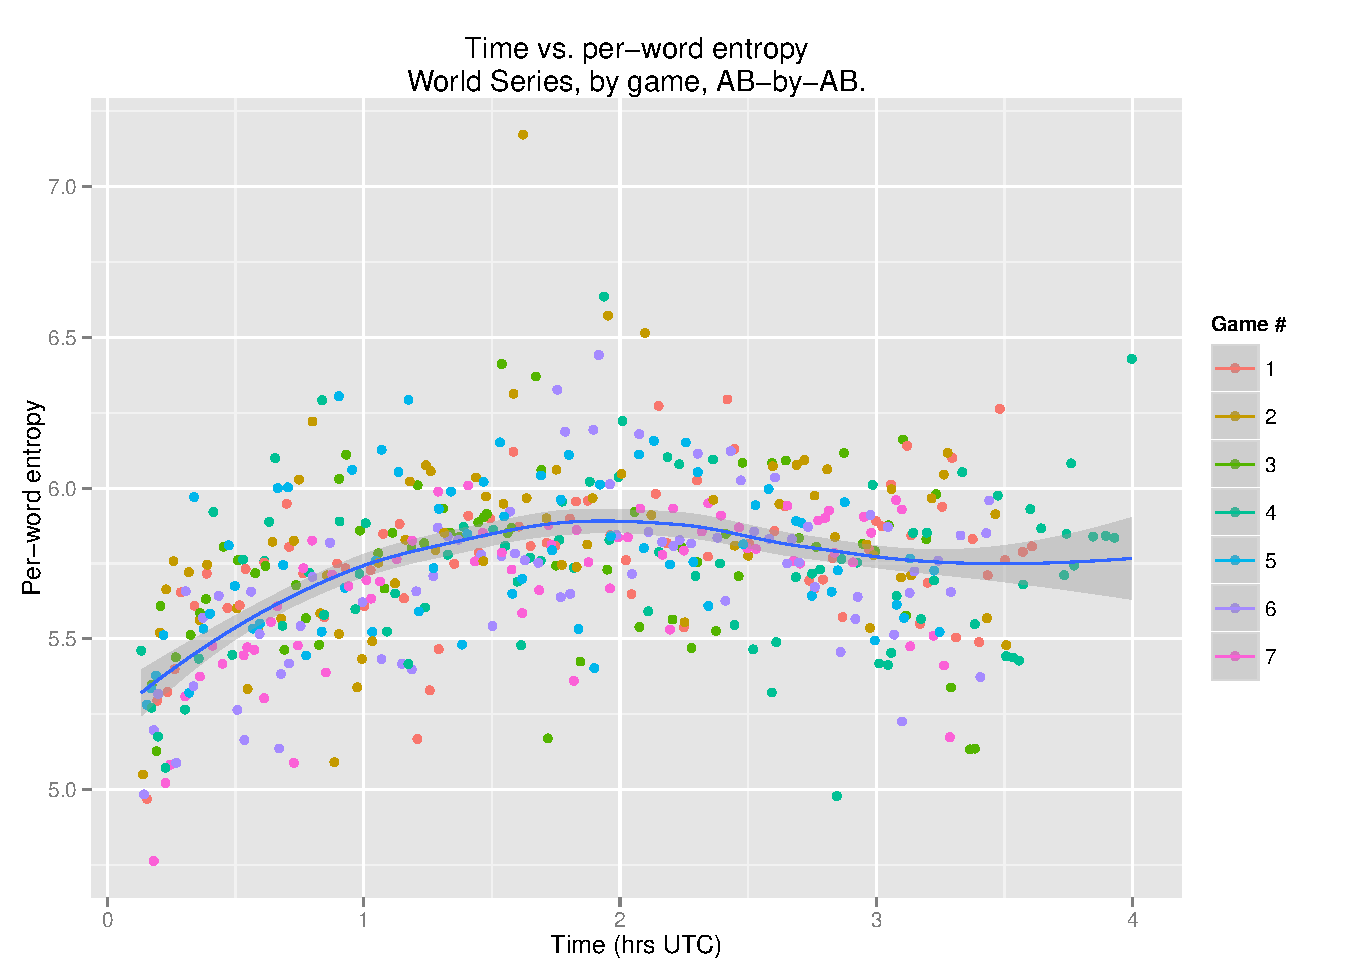
\includegraphics[width=3.25in]{figures/time-perword-ent-agg}
 \caption{Per-word entropy increases with time for the first two hours of the games, then levels off and slightly declines. Loess curve fitting with 95\% confidence intervals.}\label{fig:time-perword-ent}\vspace*{-.5em}
\end{figure}

\begin{table}
  \begin{tabular}{ccc}
minute & tweet & perword entropy \\
\hline
1 & tweet 1 & 7\\
2 & tweet 2 & 7\\
20 & hey dude & 7\\
\hline
  \end{tabular}
 \caption{Example tweets, classified by time.}\label{tab:ex}
\end{table}

Figure \ref{fig:time-perword-ent} shows evidence for changes in per-word entropy over the course of games. 
Per-word entropy rises sharply in the first half-hour of each games, then begins to level off and finally declines slightly over time.  This pattern is consistent with the constant entropy rate proposal of \cite{genzel2002}, and more specifically with the context decay model of \cite{qian2012}.\footnote{A late decline in per-word entropy also appeared in \cite{qian2012}'s analysis of Swedish.}  

A later tweet with the same in-context entropy as an earlier tweet will have a higher entropy when estimated out-of-context. We hypothesize that this finding is due to the accrual of common ground across users. As they watch more of the game, they share more referents and have stronger expectations about the shape of the game. This shared common ground licenses more complex language and more sophisticated linguistic references (see example tweets in Table \ref{tab:ex}). 

While this finding is consistent with previous work on the effect of context \cite{genzel2002,qian2012}, it expands the definition of context.  In previous work, the context came from explicit linguistic information, as it tested written paragraphs.  In the Twitter dataset, the context comes from real-world events during the games, as there is no canonical shared sequence of tweets that the tweeters can refer back to.  Contextual influences on entropy need not be explicitly linguistic.

\section{Fast Changes In Information Content}

\begin{figure}
 \centering
  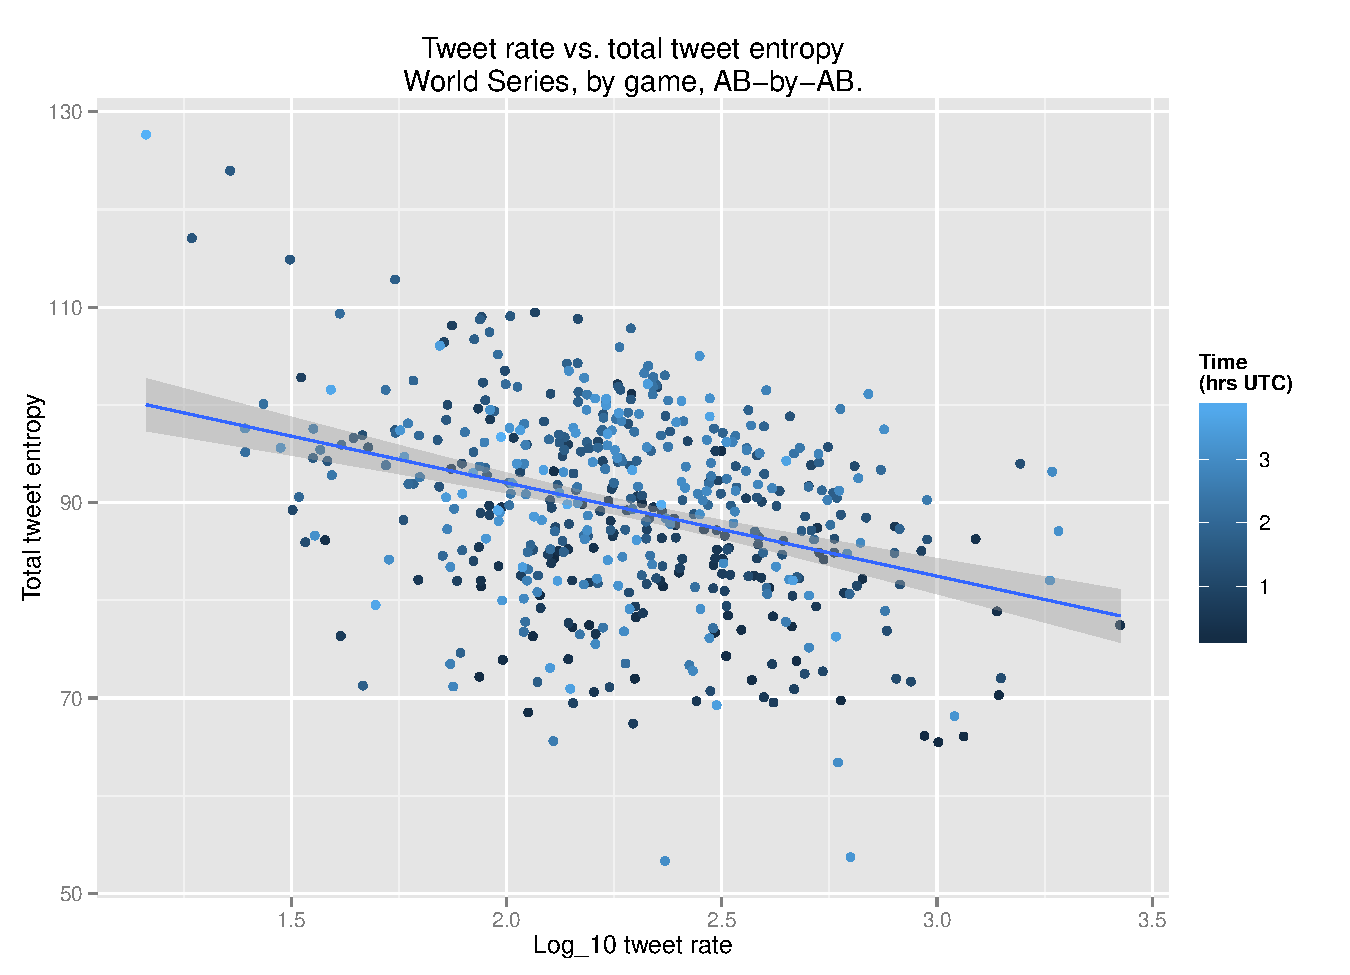
\includegraphics[width=3.25in]{figures/rate-total-ent-agg}
 \caption{Total tweet entropy plotted against log tweet rate. Color reflects in-game time; line shows the best linear fit with 95\% confidence intervals.}\label{fig:time-perword-ent}\vspace*{-.5em}
\end{figure}

\begin{table}
  \begin{tabular}{ccc}
log rate & tweet & total entropy \\
\hline
201 & tweet 1 & 7\\
10 & tweet 2 & 7\\
100 & hey dude & 7\\
\hline
  \end{tabular}
 \caption{Example tweets, classified by rate.}\label{tab:ex2}
\end{table}
Our second analytic goal was to examine fast changes in information content in response to transient in-game events. Table \ref{tab:ex2} shows some examples of tweets after high-rate and low-rate events, along with their information content. Intuitively, after an exciting, game-changing event, tweets are shorter and make mor reference to the shared knowledge that a particular event has just happened. 

This short-timescale adaptation is predicted for two reasons. First, it represents a rational response to issues of information overload, the state where the amount of incoming information exceeds a user's ability to process it \cite{miller1956}.  Previous investigations into online forum posting behavior have shown such rational responses on a longer timescale \cite{jones2001a,jones2001b,whittaker2003,schoberth2003}, as well as the more explicitly conversational setting of IRC chat channels \cite{jones2008}.  Second, given that the hashtagged tweets are tied to an ongoing real-world event, changes in tweet rates are likely to be tied to what is happening in the event, providing a potential proxy for the non-linguistic context available at the time of the tweet. We will expand on this second explanation in Section \ref{sect:other-metrics}.

This trend is reflected more strongly in total entropy (and length) than in per-word entropy. STATS

\section{Control Analyses}

\subsection{Non-Rate Metrics of Context}\label{sect:other-metrics}

\subsection{Speaker Normalization}
An alternative hypothesis for the observed behavioral changes with tweet rate is that they arise not from changes in the behavior of individuals but rather from a change in demographics.  It is plausible that rising tweet rates come from an influx of new tweeters into the hashtag, and that these new tweeters simply produce shorter, less informative tweets in general.  For instance, spambots often include trending hashtags in their spam tweets \cite{martinez2013}.

To account for this, we treat the users whose tweets are in our corpus as a ``computational focus group'' \cite{lin2013,lin2014}, and collect a further 100 tweets outside the timeframe of the game for each of them.  The mean length of these tweets is the treated as a baseline for each user, and we can use the number of characters above or below the user's average tweet length to show that the adaptations to tweet rate exist at individual level.

[Plot to come, still waiting on some users.]



\section{Discussion}


\section*{Acknowledgments}

We gratefully acknowledge the support of ONR Grant N00014-13-1-0287.

\bibliographystyle{naaclhlt2015}
\bibliography{tweetprag}

\end{document}
